\documentclass[../../lecture_notes.tex]{subfiles}

\begin{document}

\noindent There are two fundamental sub-networks within Convolutional Neural Networks (CNN).
\begin{itemize} [itemsep=0mm]
	\item convolution — local detection of features/patterns
	\item aggregation/abstraction
\end{itemize}
\noindent A CNN alternates between the two structures.\\
\\
Diagramming neurons can get complex and does not scale well; we use matrices instead.\\
\\
We define the parameters of a subnetwork of a neural network as follows:
\begin{enumerate} [itemsep=0mm]
	\item f — the filter size 
	\item $n_c$ — the number of input channels (matrices)
	\item s — the step size; how far to move the filter between iterations
	\item p — the padding; extra area around the input edge added to emphasize edge features
\end{enumerate}

\subsection*{Convolution}
\noindent Consider the example of analyzing a greyscale image; it may look like:

\begin{center}\begin{figure}[H]
	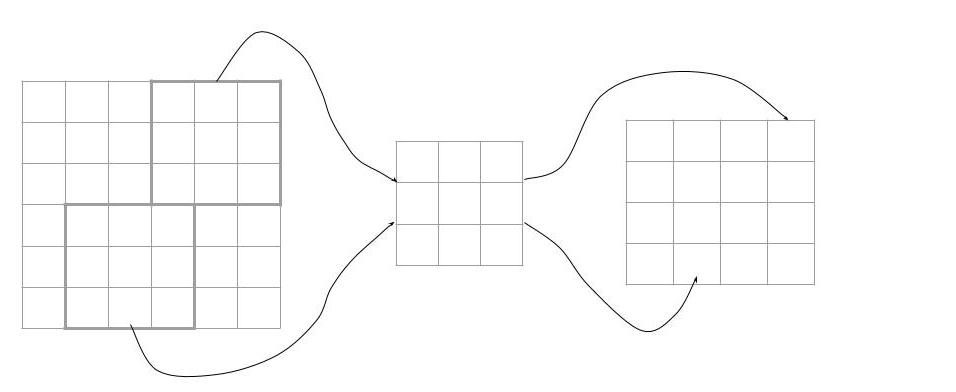
\includegraphics[scale=0.5]{convolute}
	\caption{f=3, $n_c$=1, s=1, p=0}
\end{figure}\end{center}

\noindent We pass the filter over each fxf submatrix of the input, performing a column dot product.\\
We then apply an ReLU function before entering into the output matrix.\\
The values in the filter are chosen via gradient descent.\\
We can notice that each of the hyperparameters affect the size of the output.\\
We choose these parameters heuristically, as many good models already exist.\\
The output is 4x4x1 in this example, but we could do the following transformations.
\begin{itemize} [itemsep=0mm]
	\item f++ $\to$ 3x3x1
	\item $n_c$++ $\to$ 4x4x2
	\item s++ $\to$ 2x2x1 (in this case some of the input data is ignored)
	\item p++ $\to$ 6x6x1
\end{itemize}\medskip

\noindent We can model a convolution with increased parameters like so:

\begin{center}\begin{figure}[H]
	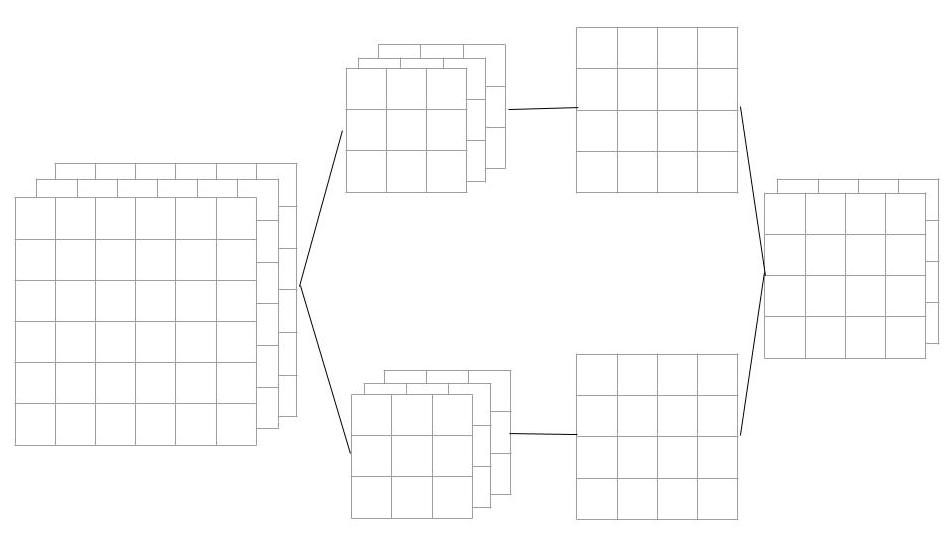
\includegraphics[scale=0.5]{2convolute}
	\caption{f=3, $n_c$=3, s=1, p=0}
\end{figure}\end{center}

\noindent This behavior may bee seen in a color (rgb) image seeking to detect two features

\subsection*{Max-Pooling}
\noindent An example may take the following form:

\begin{center}\begin{figure}[H]
	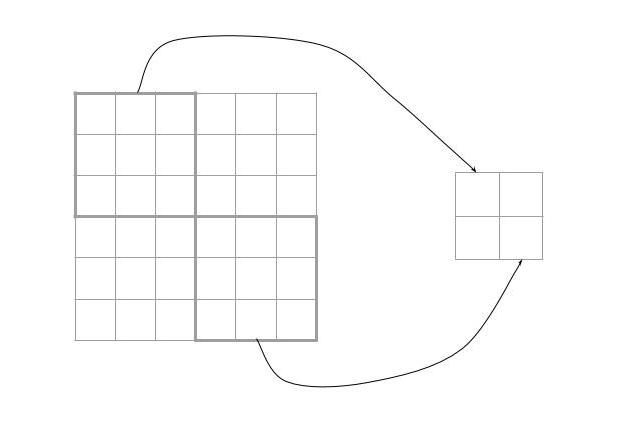
\includegraphics[scale=0.5]{maxpool}
	\caption{f=2, $n_c$=1, s=2, p=0}
\end{figure}\end{center}

\noindent The output is determined by the maximum of the values in the region it represents.\\
This effectively functions to aggregate data values to the most likely representation.\\
Padding is almost always zero, and there are no weights.\\
\\
These two operations are applied alternately to form a CNN:

\begin{center}\begin{figure}[H]
	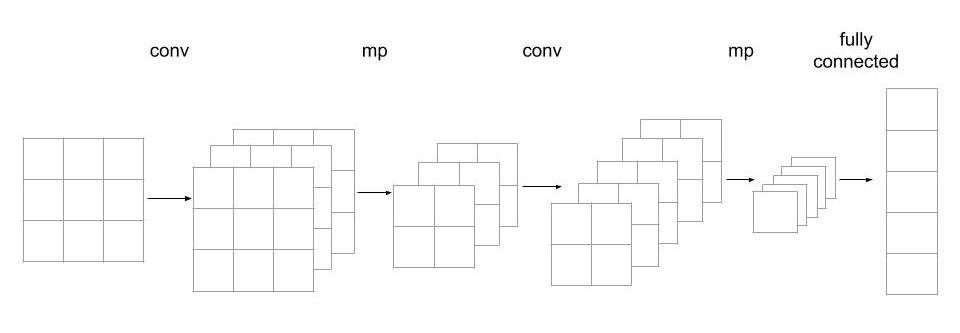
\includegraphics[scale=0.5]{neuralnetwork}
\end{figure}\end{center}

\noindent As we move right, we tend to increase filter count and thus $n_c$, but decrease f.\\
We can thus think of this operation as stretching and squishing volume in alternation.\\
The number of weights tends to be controlled and independent of the data.\\
We evaluate these with \textbf{\underline{tensors}} $\equiv$ parallelize-able multidimensional arrays.\\

\subsection*{The Future of Neural Networks}
\noindent Neural networks are intriguing because they allow us to do new things in a pretty simple way.\\
BUT people encounter issues:
	\begin{enumerate} [itemsep=0mm]
		\item data hunger\\
			this is self explanatory — neural networks require lots of labeled data to train
		\item brittleness/lack of robustness\\
			small, seemingly arbitrary changes to data can cause large output changes\\
			this leads to adversarial attacks which seek to exploit brittleness
		\item difficulty of explanation\\
			neural networks are unable to effectively explain why a certain output is correct\\
			this stems from the fact that NN are model-free and focus on function fitting
	\end{enumerate}\medskip

\noindent Here is an example of an integrated model developed in Dr. Darwiche’s lab:
The data below compares the correctness of three approaches to image recognition
	\begin{enumerate} [itemsep=0mm]
		\item Bayesian Network
		\item Bayesian Network + Background Knowledge
		\item Neural Network
	\end{enumerate}

\begin{center}\begin{figure}[H]
	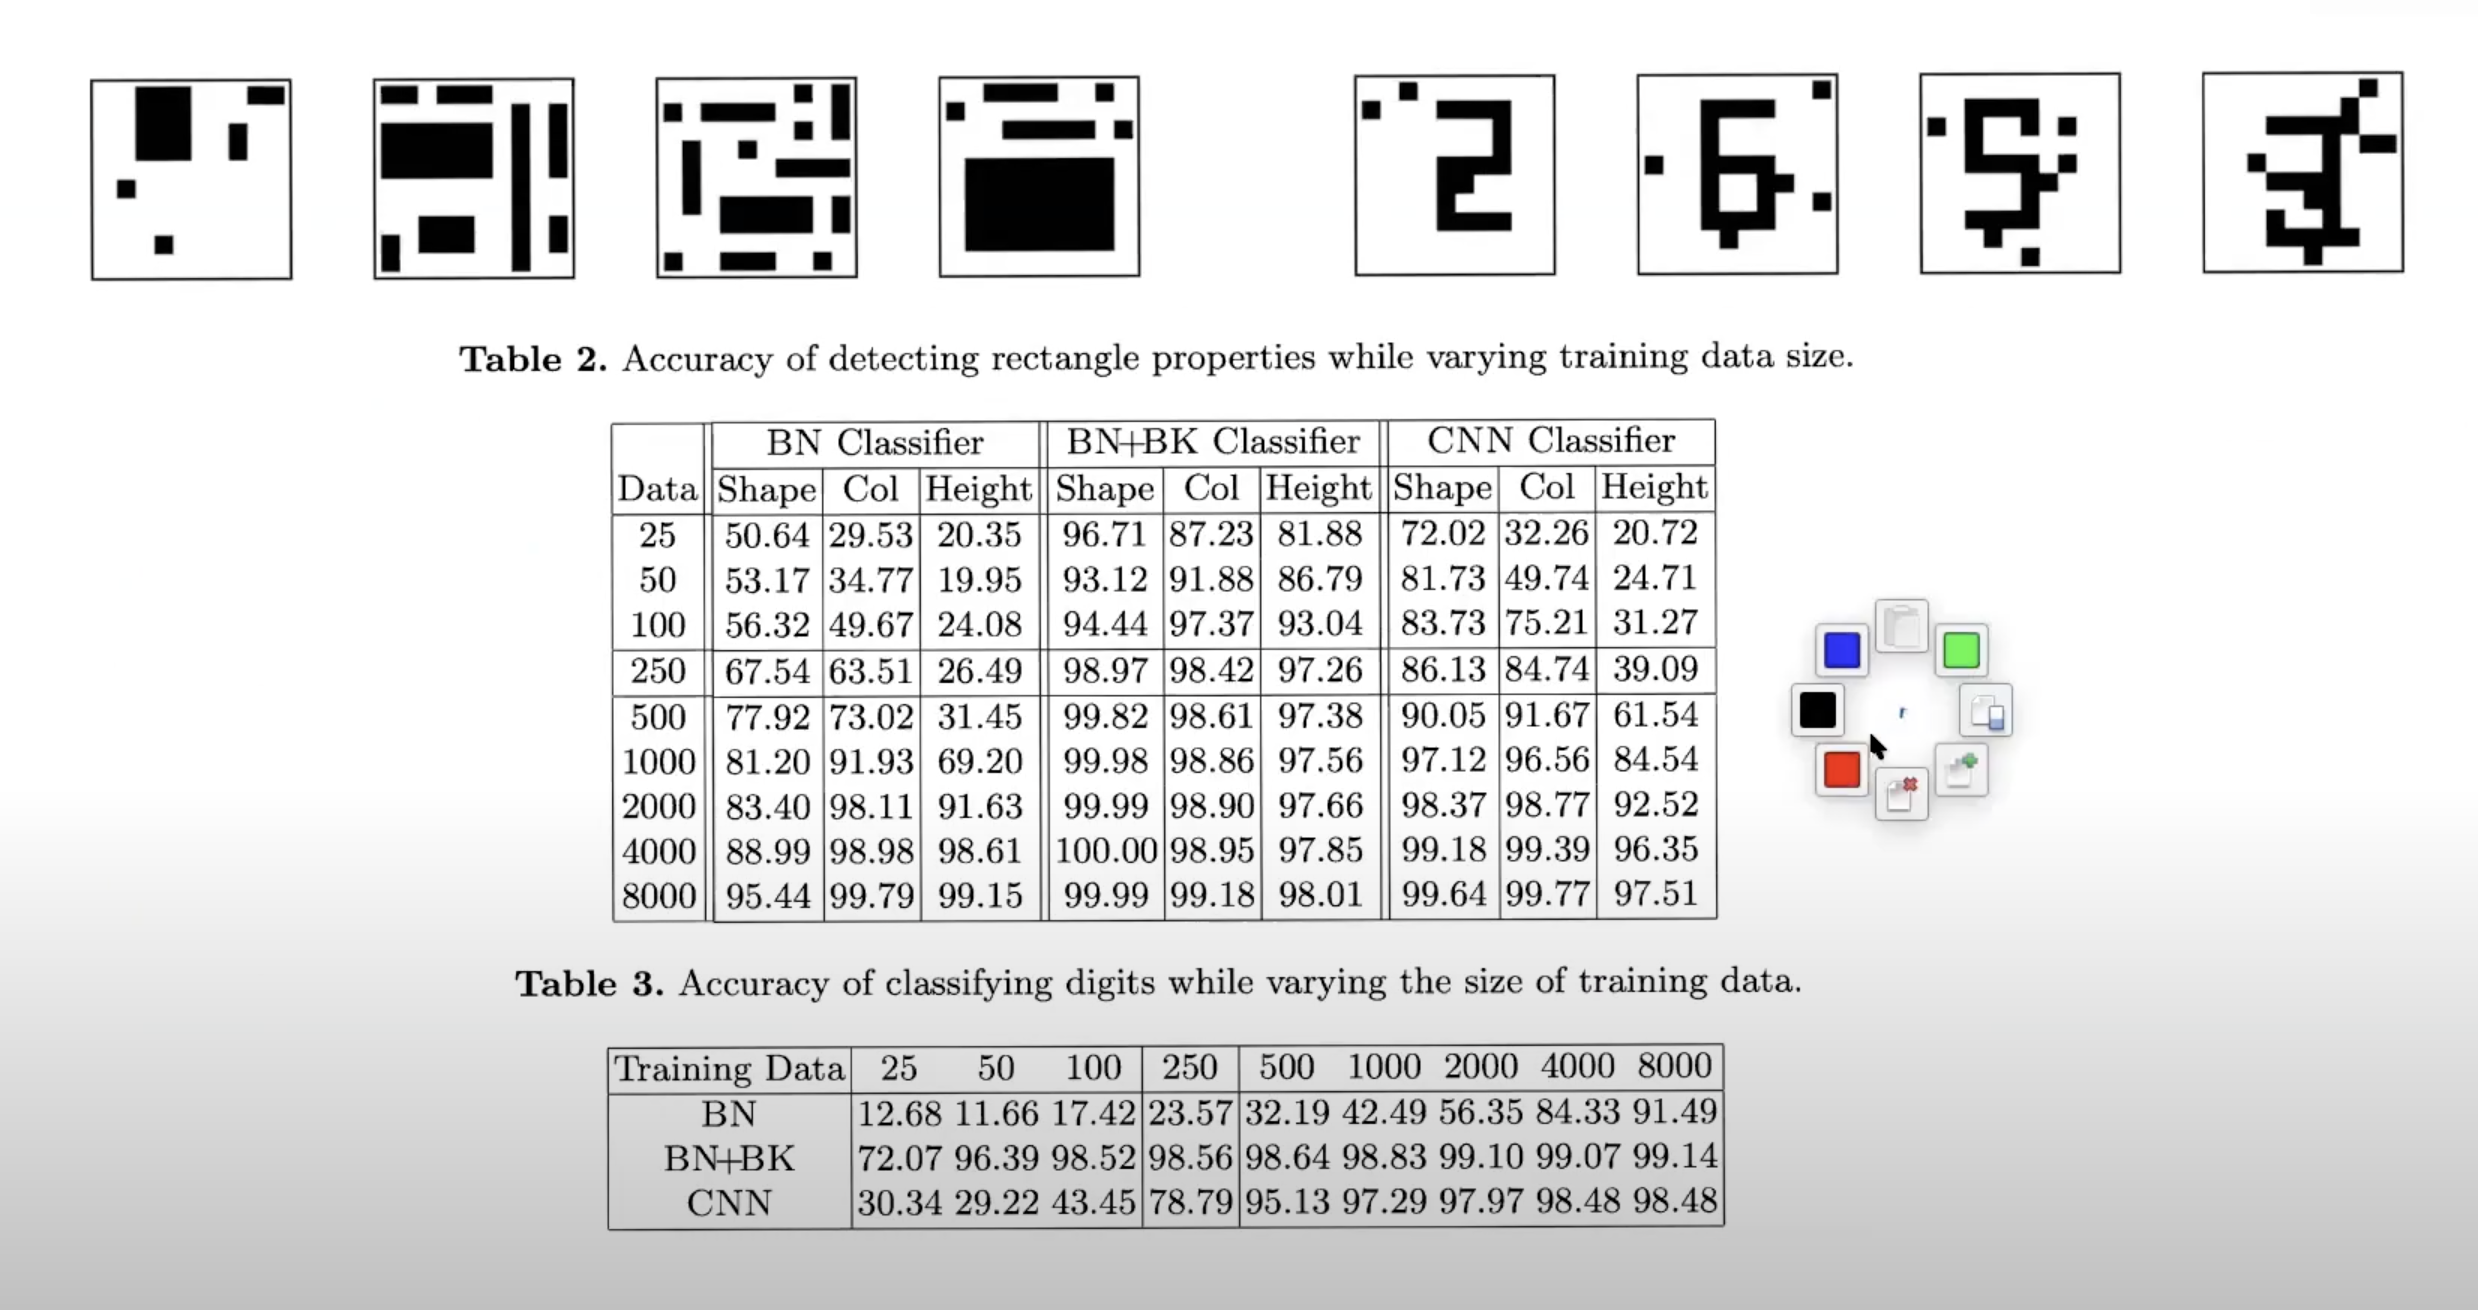
\includegraphics[scale=0.2]{comparison}
\end{figure}\end{center}

\noindent We observe that approach (b) beats the neural network handedly in low data situations.\\
Even in high data situations, approach (b) tends to beat out the neural network.\\

The below data compares the approaches when trained with different data than tested with.\\
Noise is either horizontal or vertical pairs, and the models see only one type in each.\\

\begin{center}\begin{figure}[H]
	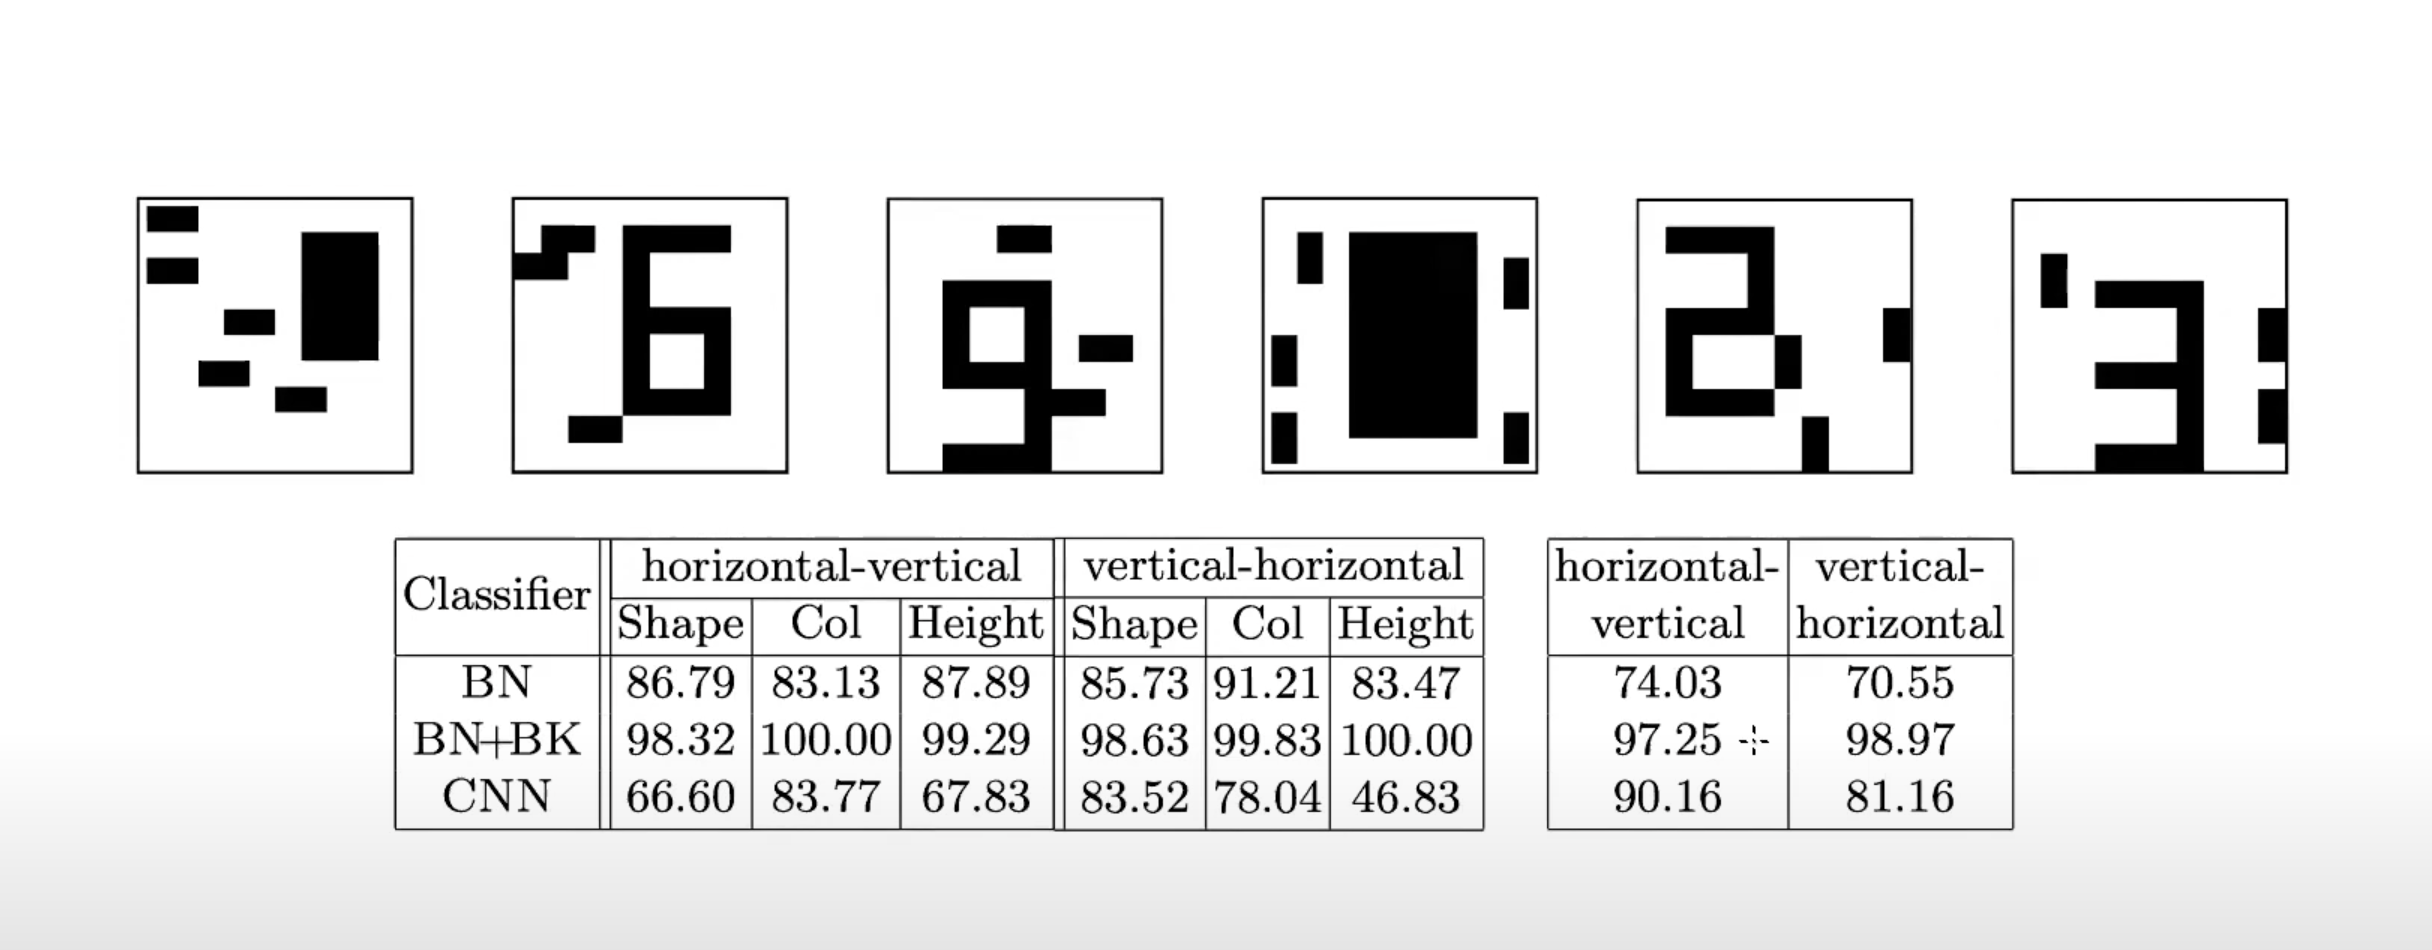
\includegraphics[scale=0.2]{orientationcomparison}
\end{figure}\end{center}

\noindent In this situation, approach (b) is relatively unaffected, but the neural network falls apart!
This is analogous to a student solving problems by applying formulae.\\
If a query represents something not well represented in the training data, an NN fails.\\
Though neural networks do very well with prototypical situations, this is impractical.\\
	\indent These type of brittleness errors are common in applications like language translators.\\
	\indent This is okay in those situations, but for higher risk thinks like self-driving cars, it is not.\\
Thus we can see that AI demands the integration of model-based and -free approaches.

\end{document}